
\chapter{Podaci i Metode} % Main chapter title

\label{Podaci i Metode} % For referencing 



\section {Podaci}

Za metode koje prezentujemo potrebne su tri vrste informacija:
\begin{enumerate}
  \item Što više različitih proteina.
  \item Pouzdana anotacija funkcija.
  \item Informacije o funkcijama, prvenstveno međurelacije.
\end{enumerate}

Međurelacije između funkcija su bitne samo ako je potrebno grupisati ih,
ili ako je potrebno mapiranje na neku drugu nomenkulaturu funkcija pa
se zahteva grupisanje.


\subsection{Podaci iz originalnog rada}

U originalnom radu \parencite{Xie2007} korišćena je  baza ručno proverenih
proteinskih sekvenci \keyword{Svis-Prot} \en{Swiss-Prot}, verzija 48 iz 2005.
Verzija 48 ima 201 560 proteina od kojih 196 326 imaju dužinu preko 40
aminokiselina (što je potrebno zbog definicije ref \ref{pdis_def}). Funkcije
pridružene proteinima izražene su \keyword{kontrolisanim vokabularom}
\en{controlled vocabulary} koga čine takozvane UniProtKB \keyword{ključne reči}
\en{keywords}. U verziji 48, UniProtKB sadrži 874 ključnih reči.  Zbog
statističke značajnost posmatrane su one ključne reči kojima je bilo anotirano
barem 20 proteina, tj. 710 ključnih reči.

Proteinske sekvence u Svis-Prot bazi ''nisu redundantne'' u smislu da 
su produkti jednog gena za jednu vrstu predstavljeni jednim entiteom 
\parencite{nonRedundant}. Zbog toga unosi u bazu tretiraju se kao proteini a ne
pojedinačne proteinske sekvence.
Međutim za analizu funkcija podaci su \keyword{statistički redundantni} jer
sadrže jako mnogo \keyword{homologih} proteina. Rešenje  klasterovati proteine
u \keyword{proteinske familije}, čime je dobijeno 27 217 familija.  Tada svaki
protein ima težinu kojom doprinosi analizi funkcija tako da je težina svih
proteina jedne familije uniformno raspoređena i sabira se na jedan.  Za detalje
konsultovati originalni rad. \parencite{Xie2007}.

\textbf{komentar:} \\
Ono što autori nisu elaborirali jeste da početni uslov od minimum 20 proteina
po ključnoj reči možda nije dovoljan. Ako pretpostavimo zarad ilustracije
normalnu raspodelu veličina klastera proteina, očekivali bi da klaster najčešće
sadrži 7 proteina. Dakle iako je 50 proteina pridruženo nekoj funkciji ona
verovatno ima pridruženih svega 7 familija proteina. Kako familija sadrži
proteine pod pretpostavkom istog evolutivnog porekla njihova funkcija bi
trebalo da je slična pa se onda postavlja pitanje da li je 7 familija dovoljno
da bi se razmatrala data ključna reč. Ovo je primarno kritika za ključne reči
jer one obično predstavljaju jako opšte pojmove.

Sa druge strane za usko specijalizovane pojmove bila bi dovoljna jedna familija
proteina jer bi ona predstavljala sve razne homologe (TODO Burkhard Rost,
Termofili)



\subsection{Naši podaci (CAFA3 proteini)}

U ovom radu korišćen je skup proteina preuzet sa \keyword{CAFA3} takmičenja gde
je korišćen kao trening skup za predikciju funkcija proteina \parencite{CAFA}.
Podaci se sastoje od dve datoteke:

\begin{enumerate}
  \item \file{uniprot\_sprot\_exp.fasta}  sadrži 41 793 proteina od kojih
         41 227 ima dužinu veću od 40 aminokiselina.
  \item \file{uniprot\_sprot\_exp.txt} pridružuje funkcije označene kao
        \keyword{GO termini} \en{Gene Ontology terms}. Postoje
        termini iz sve tri ontologije: 16 117 ćeliskih komponenti,
        5 966 molekulskih funkcija i 16 117 bioloških procesa.Jednom proteinu
        može biti pridruženo više GO termina i obrnuto.
\end{enumerate}

CAFA3 trening skup je pažljivo odabran podskp Swis-Prot proteina i smatra se da
nije \keyword{statistički redundantan} \parencite{??}. Iz tog razloga nije
potrebno vršiti klasterovanje i analiza je jednostavnija te u metodama
predstavljamo samo jednostavan oblik formula koje odgovaraju CAFA3 podacima.

Sekvence su kodirane jednim karakterom i koristeći \keyword{IUPAC} kodove.
Među proteinima bilo je sekvenci sa nestandardnim aminokiselinam 'U'
i 'O' ili višeznačnim oznakama 'B', 'J', 'X' i 'Z'. Ovi proteini se preskočeni jer
ih VSL2b predkitor ne podržava. Nakon filtiranja ostalo je 41 119 proteina.

U ovom radu analiziraćemo samo termine molekulskih funkcija.  Od 5 966 termina
svega 358 ima pridruženo 20 ili više proteina. Zbog prirode ontologija ovaj broj
se može povećati uopštavanjem termina sa malim brojem pridruženih proteina ili
obrnuto specijalizacijom onih sa velikim brojem pridruživanja. Detaljan postupak
uopštavanja i specijalizacije objašnjen je u metodama.


\section {Metod}

Cilj rada bio je ispitivanje veze između molekulske funkcije proteina i njegove
(ne)uređenosti tj.  da li ona zavisi više od uređenosti ili neuređenosti.

\textbf{Idealan slučaj.} 
Pretpostavimo da za proizvoljnu molekulsku funkciju imamo skup različitih
proteina.  Da bi dali korektan odgovor na ovo pitanje moramo da znamo kako
neuređenost pojedinačnog proteina utiče na zadatu funkciju, da li je bitna ili
nije bitna. Nije dovoljno samo posmatrati da li protein ima neuređeni region
jer možda on ne utiče na funkciju. Ovaj pristup zahteva ekspertsko poznavanje
svakog proteina i anotirane funkcije te stoga  može da se primeni na jako malo
funkcija. Takođe, trenutno svega 803 proteina ima eksperimentalno opisanu
neuređenost \parencite{disprot} 

\textbf{Realnost.} 
Možemo da damo procenu ako pretpostavimo da veći udeo neuređenih u odnosu na
uređene proteine podrazumeva da funkcija zavisi više od neuređenosti.  Dakle
ono što želimo jeste da ispitamo \keyword{korelaciju} između funkcije i
(ne)uređenosti proteina kojima je pridružena. Ali prvo potrebno je definisati
šta znači da je protein neuređen. Definicija mora da ima biološkog smisla za
analizu ali pored toga je ograničena je sposobnostima i preciznošću prediktora
koji se korist. Više o tome u nastavku.


\subsection{Predikcija dugih neuređenih regiona}

Autori \parencite{Xie2017} koristili su \keyword{PONDR VL3E} prediktor koji
postiže tačnost od $~87\%$ pri unakrsnoj validaciji nad uravnoteženim test
skupom.  Zbog ekonomičnosti i dostupnosti mi smo koristili \keyword{PONDR
VSL2b}.

Oba prediktora pripadaju \keyword{PONDR} \en{(Predictor Of Naturally Disordered
Regions)} familiji prediktora. Ovi prediktori zasnivaju se na eksperimentalno
pokazanim karakteristikama neurđenih regiona. Preciznije određene aminokiseline
verovatnije su da se jave u neuređenom regionu. Neuređeni regioni imaju manje
aromatičnih i hidrofobnih AK, veći ukupni naboj, veći indeks fleksibilnost i
manju kompleksnost sekvence. Ove osobine izražene kao atributi koriste se za
treniranje neuronske mreže \en{neural networks} sa propagacijom unapred \en
{feed forward} koja koristi prozor veličine između 9 i 21 aminokiseline.
Finalni prediktor predstavlja kombinaciju nekoliko neuronskih mreža gde je
svaka od njih trenirana nad različitim podacima specijalizujući se da predviđa
samo regione određene veličine ili položaja. PONDR familija ima nekoliko
prediktora koji  se razlikuju u načinu treniranja što se postiže kombinacijom
različitih trening skupova.  Oznaka ''VSL2b'' kodira tipove proteinskih skupova
nad kojima su trenirani prediktori.
\begin{itemize}
  \item V - Opisuje eksperimentalnu tehniku kojom je neurđenost utvrđena na
    trening skupu \en{X-ray, NMR, circular dichroism}
  \item S - Prediktor je treniran na skupu proteina sa \keyword{kratkim}
      neruređenim
    regionim ($<30$ AK)
  \item L - Prediktor je treniran na skupu proteina sa \keyword{dugim}
    neuređenim regionima ($>30$ AK)
\end{itemize}

VSL2b kao ulaz prima proteinsku sekvencu minimalne dužine 9 AK kodiranih jednim
karakterom. Podržava azbuku od samo 20 standardnih AK.  Izlaz je niz
ocena(verovatnoća) za svaku aminokiselinu da li pripada neuređenom regionu to
jest da je taj rezidual
\footnote{ Rezidual je čest naziv koji se koristi za elemente na nekoj
  poziciji sekvence.  Koristi se za aminokiseline  proteina ali i za nukleinske
  kiseline kod DNK i RNK.  Naziv potiče od hemiskih tehnika prečišćavanja čiji
  su rezultati reziduali (ostaci).
} neuređen. Reziduale sa vrednošću iznad 0.5 smatramo neuređenim a suprotno
uređenim. Za potrebe analize autori uvode sledeću definiciju:\\

\newtheorem{mydef}{Definicija}
\begin{mydef}
\label{pdis_def}
Protein je \keyword{verovatno/putativno neuređen} \en {putatively disordered} ako
sadrži bar jedan region veći ili jednak od 40 uzastopnih aminokiselina
takvih da imaju \textit{predviđenu neuređenost} iznad 0.5. \\
\end{mydef}

Onda definišemo operator $d$ takav da za svaku proteinsku sekvencu $s_i$ važi:


\[   
  d(s_i) = 
    \begin{cases}
      1 & \text{ako je} \quad s_i \quad \keyword{verovatno neuređena}\\
      0 & \text{suprotno}
    \end{cases}
\]


\subsection{Zavisnost dužine proteina i predikcije dugačkog neuređenog regiona}

Verovatnoća da po gornjoj definiciji protein bude klasifikovan kao verovatno
neuređen raste sa porastom njegove dužine. Ovo je ozbiljan problem koji utiče
na statističku značajnost rezultata. Autori \parencite{Xie2007} predstavljaju način
da se ta verovatnoću proceni.
Označimo tu verovatnoću sa $P_L$ gde $L \in N$ označava dužinu sekvence. Neka
je $V_L$ skup svih validnih proteina dužine $L$ onda bismo $P_L$ mogli da
procenimo kao količnik broja verovatno neuređenih proteina iz $V_L$ i ukupnog
broja proteina u $V_L$. Ovaj idealan slučaj nije realan jer skup svih
validnih proteina nije poznat. Pod validnošću podrazumevamo da se protein
javlja prirodno kao produkt evolucije (tj. ima ili je imao funkciju u
organizmu). Skup $V_L$ aproksimiraćemo  skupom svih naših proteina. Međutim,
ovaj skup je suviše mali i $P_L$ sadrži mnogo šuma. Da bi uglačali rezultat
autori \cite{Xie2007} predlažu da se umesto skupa proteina egzaktne dužine $L$
koristi skup  proteina u oznaci $S_L$ sa dužinama između $[L-l, L+l]$ gde je $l
= 0.1*L$. Dobijamo sledeće formule:

$$ S_L = \{s_i \mid \quad | L -  \Vert s_i \Vert | <= l \quad   \}$$
$$ P_L = \dfrac{ \sum_{s_i \in S_L} d(s_i)} {\Vert S_L \Vert}$$

Ponašanje $P_L$ predstavljeno je na grafiku \ref{fig:PL1}. Glatkoća rezulatata
kontroliše se veličinom $l$ koja predstavlja prozor uprosečavanja. Kako je $l =
0.1*L$ tako da prozor uprosečavanja raste sa porastom dužine proteina te $P_L$
postaje glađe sa veličinom proteina. Za konstantni prozor uprosečavanja ova
tehnika je još poznata kao \en{rolling average} ili \en{boxcar filter} i
pripada specijalnoj vrsti konvolucije. Trenutno ne znamo zašto se autor odlučio
da veličina prozora raste sa dužinom proteina.


\begin{figure}[th]
\centering
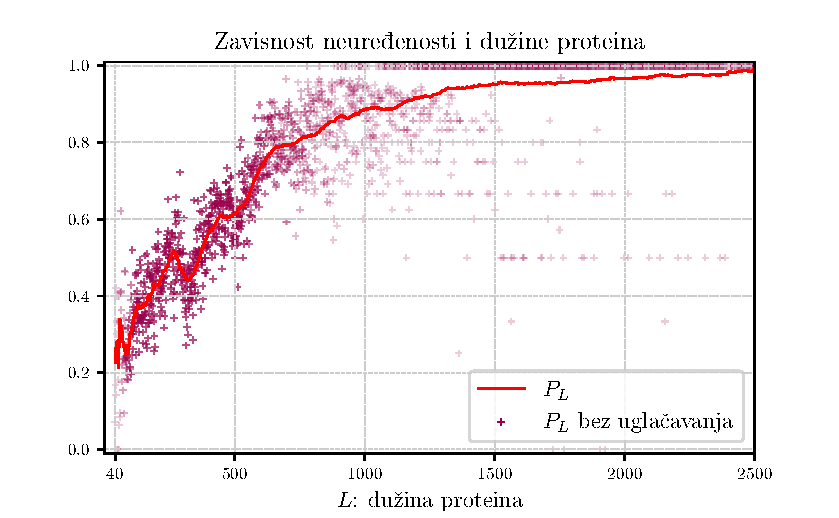
\includegraphics[]{../plots/PL_F}
\decoRule
\caption {
 Punom linijom predstavljena je $P_L$ sa prozorom uprosečavanja $l = 0.1L$,
 a krstići predstavljaju sirove vrednosti $l = 0$ 
}
\label{fig:PL1}
\end{figure}


Pored gore prikazanog 'originalnog' metoda predstavljamo još jedan pristup.
\keyword{Slučajno generisani} \en{random generated} proteini za procenu $P_L$.
Razmotrićemo dva modela. Prvi je naivan model \keyword{uniformne verovatnoće}
koji podrazumeva da se svaka aminokiselina javlja sa istom verovatnoćom odnosno
$1/20$. U statistici ovo je još poznato kao \en{equiprobable model}.  Drugi
model koji ćemo zvati 'slučajni' ili 'random' model predstavlja slučajnu
promenljivu čija verovatnoća zavisi od učestalosti aminokiselina iz CAFA3 skupa
i prikazana je na grafiku \ref{fig:ucestalost_AK}.  Koristeći ova dva modela za
svaki protein generisan je slučajan protein iste dužine koji se koristi za
procenu $P_L$.


\begin{figure}[th]
\centering
% \includegraphics[scale=0.7]{Figures/ucestalost_AK}
\includegraphics[]{../plots/ucestalost_AK}
\decoRule
\caption{Učestalost aminokiselina u podacima}
\label{fig:ucestalost_AK}
\end{figure}



Poređenje ova dva pristupa sa originalnim $P_L$ prikazano je na slici
\ref{fig:PL2}.  Originalni $P_L$ ostaje prikazan kao puna linija. Jasno se vidi
da slučajni model prikazan isprekidanom linijom predstavlja vizuelno dobru
aproksimaciju dok uniformni model verovatnoća prikazan tačkicama znatno odstupa
i dosta sporije raste (reklo bi se skoro linearno). Kako VSL2b predkitor
prepoznaje neuređene regione na osnovu učestalosti aminokiselina ovo ponašanje
nije čudno jer je manja verovatnoća pojave aminokiselina koje promovišu
neuređenost. Zbog suviše velikog odstupanja uniformni model nije korišćen u
daljoj analizi.


\begin{figure}[th]
\centering
% 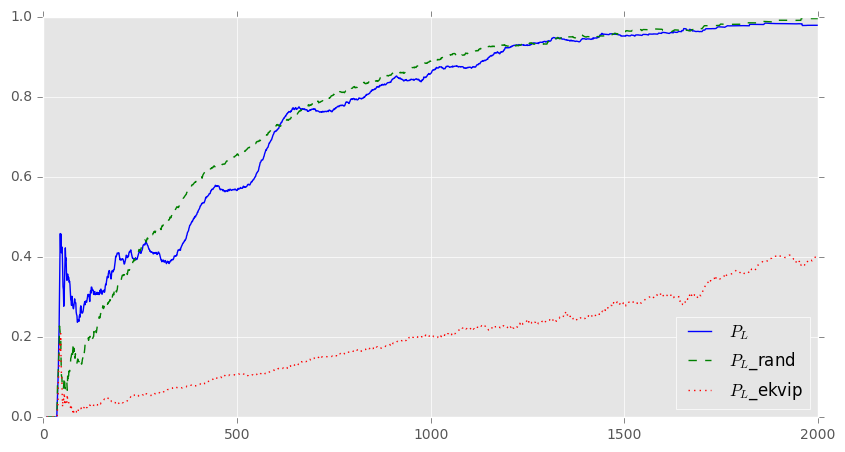
\includegraphics[scale=0.65]{Figures/PL2}
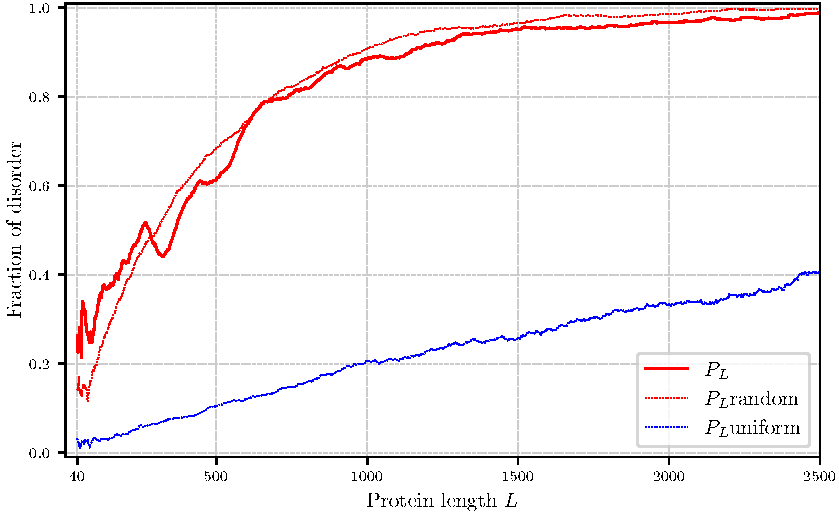
\includegraphics[]{../plots/PL_F_cmp}
\decoRule
\caption{Različiti pristupi za procenu $P_L$}
\label{fig:PL2}
\end{figure}


Jedno objašnjenje zašto je uniformni model naivan i toliko odstupa od
prvobitnog metoda proizilazi iz činjenice da aminokiseline imaju inherentno
različite verovatnoće. Naime  aminokiseline ne mogu  imati istu
verovatnoću jer se  broj njihovih kodona razlikuje. Neke aminokiseline
su kodirane sa samo jednim a druge i sa 6 kodona. Očekivali bi da broj kodona
povećava učestalost aminokiseline i ta korelacija uz izuzetke arginina se vidi
na slici
\ref{fig:aminoacid} \parencite{AKfrekvencija}.

\begin{figure}[th]
\centering
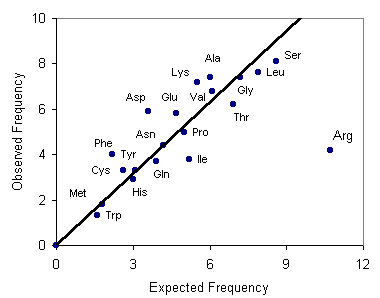
\includegraphics[scale=0.7]{Figures/aminoacid}
\decoRule
\caption{očekivana i realna učestalost  aminokiselina kod sisara}
\label{fig:aminoacid}
\end{figure}



\subsection{Ocenjivanje zavisnosti funkcije od neuređenosti}

Neka je $S_j$ skup proteina koji imaj pridruženu funkciju $j$. Tada procenat
verovatno neuređenih proteina $F_j$ možemo izračunati kao: $$F_j =
\dfrac{\sum_{s_i \in S_j} d(s_i)} {\Vert S_j \Vert} $$

Nultu hiptezu koja predviđa da je rezultat $F_j$ posledica samo slučajnosti to
jest zavisi samo od $P_L$ opisaćemo preko slučajne veličinu $Y_j$.  $$ Y_j =
\dfrac {\sum_{s_i \in S_j} {X_{|s_j|}}}{\Vert S_j \Vert}$$ Gde je $X_L$
Bernulijeva slučajna veličina sa verovatnoćom $P(X_L = 0) = P_L$ odnosno $P(X_L
= 1) = 1-P_L$

Ako $F_j$ izlazi iz intervala poverenja raspodele $Y_j$ onda funkcija $j$
sadrži značajno mnogo predviđenih neuređenih ili uređenih proteina. Preciznije
ako je \textit{p-value} $<0.05$ funkcija $j$ je povezana sa neuređenim
proteinima a ako je \textit{p-value} $>0.95$ funkcija $j$ je povezana sa
uređenim proteinima. Suprotno ne možemo ništa da tvrdimo za funkciju $j$.

$Y_j$ je teško izračunati analitički tako da se pribegava empiriskom
računanju p-vrednosti. Empiriska p-vrednost se određuje tako što se za 1000
realizacija gleda frakcija koliko puta je realizovano  $Y_j$ bilo veće od
$F_j$.
Za veće skupove $S_j$ raspodela $Y_j$ liči na normalnu pa računanjem očekivanja
$\mu_j$ i standardne devijacije $\delta_j$ za raspodelu $Y_j$ možemo da
izračunamo Z-skor kao $Z_j=(F_j-\mu_j)/\delta_j$. Dalje p-vrednost možemo da
aproksimiramo kao $1/2(1-erf(Z_j/2)))$ ako raspodela liči na normalnu.  Ovo je
nekad korisno jer sa 1000 realizacija $Y_j$ nemamo dovoljnu preciznost da
računamo p-vrednost veću ili manju od 0.01 i 0.99. Ipak koristićemo samo
empiriski izračunatu p vrednost.

\section {uopštavanje, grupisanje  GO termina}

\section {Metod za upoređivanje rezultata}
